% This is a file that contains the tracking of the activities related to the project during the first week of March 2025.
% The activities are divided into groups and a summary of the progress is provided.

\documentclass[12pt]{article} % 12pt font size
\usepackage[a4paper, margin=1in]{geometry} % Adjust margins

\usepackage{graphicx}
\usepackage{dirtree}
\usepackage{hyperref}
\usepackage[most]{tcolorbox}

\begin{document}
\author{Joan Ronquillo}

\title{Project Progress - Week 1 of March 2025}
\maketitle

This is a file that contains the tracking of the activities related to the Hydrodynamic
Interactions project during the first week of March 2025. The activities are divided into
groups and a summary of the progress is provided.

\section{Initial Status of the Project}
The project has made significant progress up until the first week of March 2025. The key achievements include:

\begin{itemize}
    \item Meetings with Raúl to discuss the hydrodynamic interactions.
    \item Documentation in Notion of the basic theory behind hydrodynamic interactions.
    \item Preliminary exploration of the "spreadinterp" repository.
    \item Creation of a general function to obtain the mobility tensor given a solver and a set of particle positions.
    \item Initial tests for obtaining the "Self-Mobility Tensor".
\end{itemize}

\section{Potential Tasks for the Week}
The following tasks have been identified as potential areas of focus for the first week of March 2025:
\begin{itemize}
    \item Development of the Python module with the implementation functions.
    \item Tests for obtaining the RPY tensor. Discussion of the representation and its properties.
    \item Initial functions to establish specific particle arrangements and geometries.
\end{itemize}

\section{Week Tracking}
\subsection{Monday - March 3, 2025}
The repository has been reorganized, and the functionalities of \path{.gitignore}, \path{setup.py},
and \path{__init__.py} have been discussed to manage the import of functions and modules. 
The use of pytest and the inclusion of asserts in the test functions are emphasized. 
The correct functioning of the self-mobility tensor test is verified.

\subsection{Tuesday - March 4, 2025}
I have been learning how to compile LaTeX projects located inside the repository.
The pdf tab viewer in VSCode has been installed and configured to facilitate the 
visualization of the documents. This document serves as an example of the compilation 
process.

\subsection{Wednesday - March 5, 2025}
The tasks for the week have been specified and the progress in documentation, code, and testing has been tracked.
The script \path{test/test_RPY_distance.py} has been created to obtain 
the RPY mobility for two particles as a function of the distance 
between them. The script checks the symmetry of the tensor, the 
reproduction of the self-mobility elements on the diagonal, the 
symmetry of the elements of the off-diagonal blocks of cross mobility,
the nullity of the elements corresponding to crossed coordinates 
(the particles are on the x-axis), and the equivalence between the 
two yy, zz terms (perpendicular to the axis that joins the particles) 
of the cross mobility diagonal. The script also generates a graph
with the dependence of the non-zero elements of the cross mobility
with the distance between the particles, from 0.1 to 10 times the
hydrodynamic radius of the particles. The ordering and storage of
this type of graphs in the repository must still be studied.

\subsection{Thursday - March 6, 2025}
Added checks to the test file \path{test_RPY_distance.py} that
include the equivalence between the analytical result and the matrix
obtained in the numerical calculation. The code has been refactored
to separate functions, with one function for generating the graph and
another for the array of analytical tensors. Additionally, the
\path{output/} directory has been created to store the graphs generated
by the test scripts.
\begin{figure}[h]
    \centering
    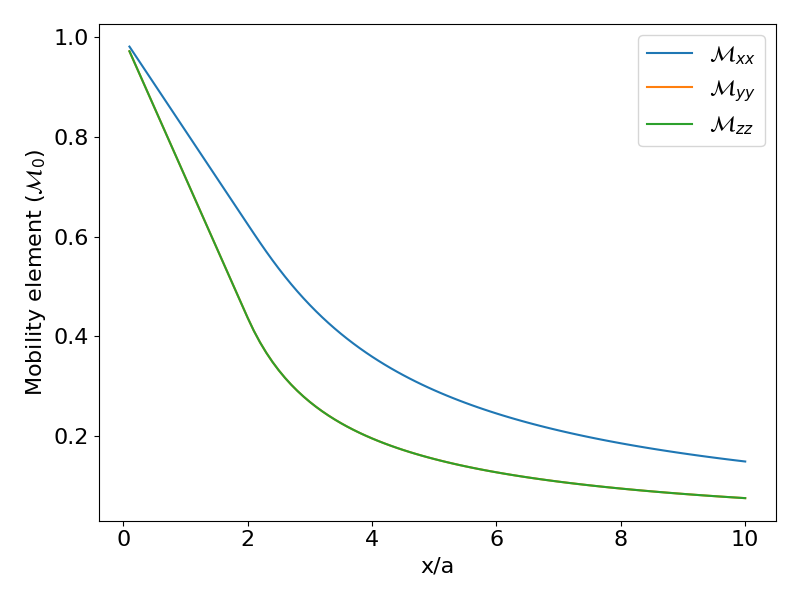
\includegraphics[width=0.8\textwidth]{figures/RPY_mobility_tensor_distance_dependence_.png}
    \caption{RPY mobility for two particles as a function of the distance between them.}
    \label{fig:RPY_mobility_tensor_distance_dependence}
\end{figure}
The figure shown in Figure \ref{fig:RPY_mobility_tensor_distance_dependence}
depicts the RPY mobility for two particles as a function of the distance
between them. The mobility decreases with distance, decaying exponentially
when the particles do not overlap. It can be observed that the mobility is
higher in the direction of the line connecting the particles and lower in
the perpendicular directions. When the particles overlap, the mobility
decreases linearly with distance. In the case of complete overlap where
the particles are in the same position, the mobility is the same as the
self-mobility of an isolated particle. No singularities in the mobility
are observed in the case of complete overlap.

\begin{tcolorbox}[colback=blue!5!white, colframe=blue!20!black, title=Doubt, colbacktitle=blue!20!white, coltitle=black]
    What does the overlap of the particles mean?
\end{tcolorbox}

\subsection{Friday - March 7, 2025}
The plot functionality has been removed from the testing code,
as discussed with Raúl regarding the convenience of creating plots
in non-testing scripts. Additionally, emphasis has been placed on
the importance of building good function interfaces (declarations,
arguments, and returns) that simplify and minimize complexity for
ease of use and scalability. A meeting with Rafa was held to provide
an overview of the current project status, with a focus on tasks such
as creating specific particle configurations and geometries,
particularly the configuration of a sphere near a horizontal wall
(potentially a liposome system). The idea is to apply an external
force to the sphere and observe its displacement and deformation.
This can be useful for future treatment of surface interactions
and the modes of vibration of an immersed or nearby liposome in
relation to a surface, as well as the decomposition of forces and
velocities in the basis of vector spherical harmonics.

\section{Next week tasks}
The next steps for the project include:
\begin{itemize} 
    \item Modification of the structure of the \path{get_mobility_tensor} function, establishing default arguments and eliminating external initialization.
    \item Reading of Raúl's documents on software development.
    \item Exploration/creation of Python functions that allow specific particle arrays and geometries to be established.
    \item Exploration/creation of Python functions that handle vector spherical harmonics (VSH) and their properties. Study of the convenience of a class.
    \item Creation of Python functions that allow the mobility tensor to be obtained in the basis of VSH.
    \item Brennan's paper reading.
\end{itemize}
\end{document}
